\documentclass[a4paper,11pt]{article}
\usepackage{graphicx} % Required for inserting images
\usepackage{lipsum}
\usepackage{amsmath}
\usepackage{biblatex}
\usepackage{booktabs}
\addbibresource{bibn.bib}
\title{Rapport Numerical Tours}
\author{Romain Gambardella}
\date{January 2025}

\begin{document}

\maketitle

\section{NT 1 : Optimal transport maps}

For this Numerical tour, I chosed to study numerically the convergence of the Wasserstein-2 distance beetween two sampled gaussian distributions.

This means, for each $n$ we define the random discrete distributions $a_n(w) = \frac{1}{n} \sum{\delta_v(X(w))}$ and  $b_n(w) = \frac{1}{n} \sum{\delta_v(Y(w))}$ where $X$ and $Y$ follow a Gaussian law centered at the origin and with identity covariance matrix. Then, I studied the empirical Wasserstein distance $D_n(w) := W_2(a_n(w), b_n(w))$ and it's convergence properties when $n \rightarrow \infty$.

As we know that $a_n$ and $b_n$ converges weakly to $N(0,I_2)$ $w-p.s$, we have that a.s. $D_n \rightarrow 0$ when n tends to infinity.

Moreover, it is shown in \cite{Dud} that the rate of convergence of the mean of the absolute error ( in our case of $\mathbf{E}(D_n)$ ) should be in $O(n^{-\frac{1}{d}})$, for any $d >2$, and the bound should be tight here as the measures admits density w.r.t the Lebesgue mesure. Our goal is to reproduce numerically these convergence rates.

\subsection{Toy example : distance beetween sampled gaussians in 2D}

To illustrate our case, let us set ourselves in dimension 2. We can plot easily using cvxpy the optimal matching beetween two Gaussian distributions, sampled with a varying number of points $n$ ( see \ref{fig:enter-label} ).

\begin{figure}
        \centering
        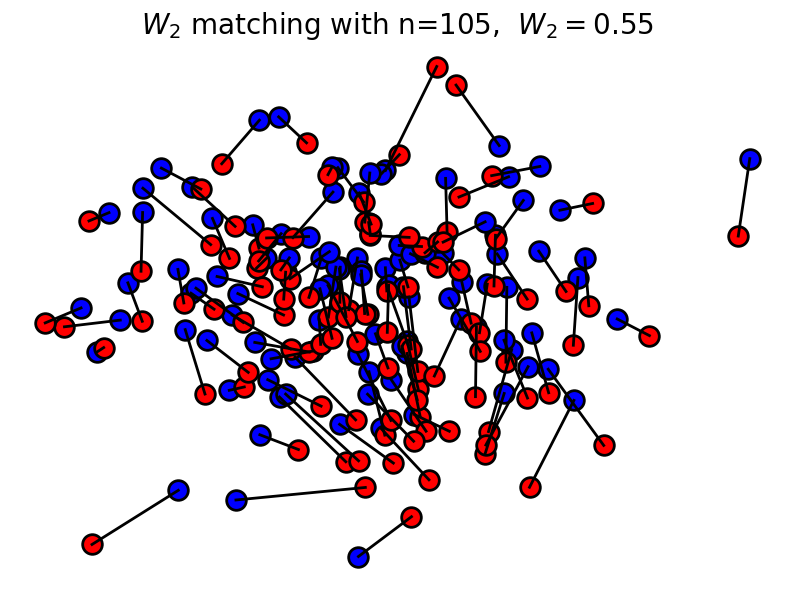
\includegraphics[width=0.45\linewidth]{image/n105.png}
        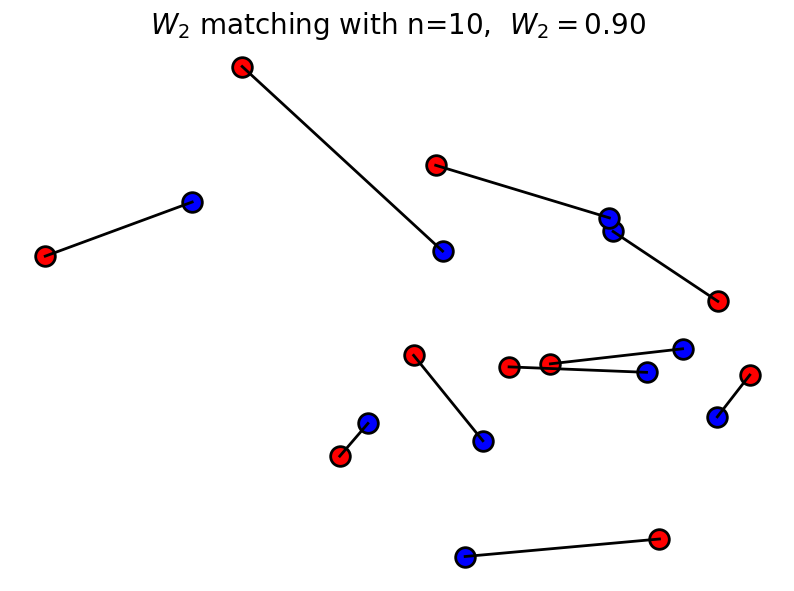
\includegraphics[width=0.45\linewidth]{image/n10.png}
        \caption{Optimal transport matching for the $L_2$ norm}
        \label{fig:enter-label}
    \end{figure}

\subsection{Evolution of the error as the number of point evolves}

Then, we can plot the evolution of the $W_2$ distance beetween $a_n$ and $b_n$ as the number of point increases ( see \ref{fig:2}. For each number of points $n$, we sample 5 times $a_n$ and $b_n$ in order to get unbiased estimators of the mean ( represented in dark blue ) of the r. v. $W_2(a_n, b_n)$.

We clearly see on the log plot ( the log is both on the x axis and on the y axis ) that, as expected theoritically, the curves follow a straight line. By linear regression, we can compute the slope of the curves. In the table \ref{tab:slope_vs_n} we see that the theoritical results completly agree with the experiment.

\begin{figure}
    \centering
    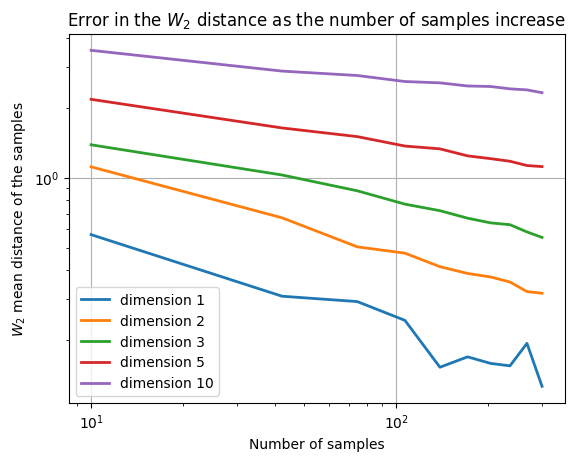
\includegraphics[width=0.8\linewidth]{image/123510logconv.png}
    \caption{$W_2(a_n, b_n)$ in dimension 1, 2, 5  in logx logy plot}
    \label{fig:2}
\end{figure}
\begin{table}[h!]
\centering
\begin{tabular}{ccc}
\toprule
$d$ & Slope & Theoretical Slope \( -\frac{1}{d} \) \\
\midrule
1  &-0.41 & ? \\
2  &-0.36 & ? \\
3  &-0.27 & -0.33 \\
5  &-0.20 & -0.20 \\
10 &-0.11  & -0.10 \\
\bottomrule
\end{tabular}
\caption{Slope as a function of \( d \) along with the theoretical slope \( \frac{1}{d} \)}
\label{tab:slope_vs_n}
\end{table}

\section{NT 2 : Entropic regularisation of Optimal Transport}

For this Numerical tour, I chosed to apply the Wasserstein barycenter on images from the MNIST dataset.

For this, I first loaded MNIST images and thresholded them in order to get images with value in {0,1}, then I normalized them and applied the Wasserstein Barycenters algorithm.

Then, I plotted the Wasserstein Barycenter for varying weights to get the images \ref{fig:mnist}.
\begin{figure}
    \centering
    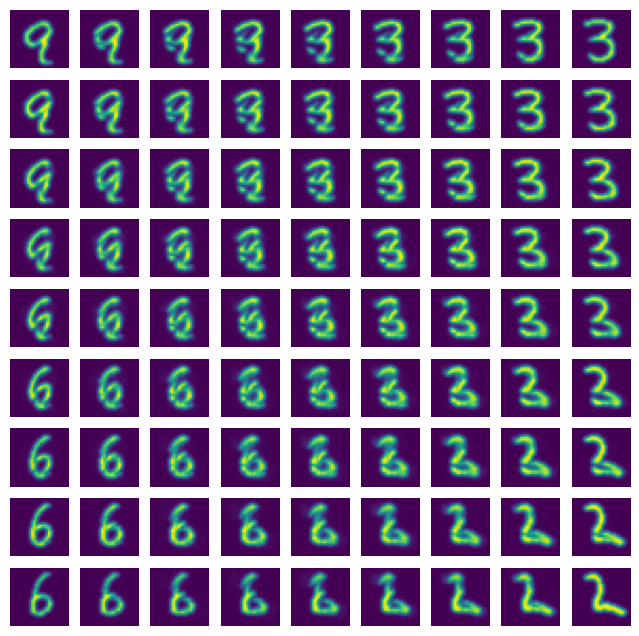
\includegraphics[width=0.75\linewidth]{image/MNIST_barycenter.png}
    \caption{Wasserstein Barycenter on the MNIST dataset}
    \label{fig:mnist}
\end{figure}

\newpage
\printbibliography
\end{document}